%%%%%%%%%%%%%%%%%%%%%%%%%%%%%%%%%%%%%%%%%
% Thesis 
% LaTeX Template
% Version 2.5 (27/8/17)
%
% This template was downloaded from:
% http://www.LaTeXTemplates.com
%
% Version 2.x major modifications by:
% Vel (vel@latextemplates.com)
%
% This template is based on a template by:
% Steve Gunn (http://users.ecs.soton.ac.uk/srg/softwaretools/document/templates/)
% Sunil Patel (http://www.sunilpatel.co.uk/thesis-template/)
%
% Template license:
% CC BY-NC-SA 3.0 (http://creativecommons.org/licenses/by-nc-sa/3.0/)
%
%%%%%%%%%%%%%%%%%%%%%%%%%%%%%%%%%%%%%%%%%

%----------------------------------------------------------------------------------------
%	PACKAGES AND OTHER DOCUMENT CONFIGURATIONS
%----------------------------------------------------------------------------------------

\documentclass[
11pt, % The default document font size, options: 10pt, 11pt, 12pt
%oneside, % Two side (alternating margins) for binding by default, uncomment to switch to one side
english, % ngerman for German
singlespacing, % Single line spacing, alternatives: onehalfspacing or doublespacing
%draft, % Uncomment to enable draft mode (no pictures, no links, overfull hboxes indicated)
%nolistspacing, % If the document is onehalfspacing or doublespacing, uncomment this to set spacing in lists to single
%liststotoc, % Uncomment to add the list of figures/tables/etc to the table of contents
%toctotoc, % Uncomment to add the main table of contents to the table of contents
%parskip, % Uncomment to add space between paragraphs
%nohyperref, % Uncomment to not load the hyperref package
headsepline, % Uncomment to get a line under the header
%chapterinoneline, % Uncomment to place the chapter title next to the number on one line
%consistentlayout, % Uncomment to change the layout of the declaration, abstract and acknowledgements pages to match the default layout
]{Report} % The class file specifying the document structure

\usepackage[utf8]{inputenc} % Required for inputting international characters
\usepackage[T1]{fontenc} % Output font encoding for international characters

\usepackage{mathpazo} % Use the Palatino font by default

%\usepackage[backend=bibtex,style=authoryear,natbib=true]{biblatex} % Use the bibtex backend with the authoryear citation style (which resembles APA)

\usepackage[backend=bibtex, natbib=true, sorting=none]{biblatex} % Use the bibtex backend with the authoryear citation style (which resembles APA)

\addbibresource{example.bib} % The filename of the bibliography

\usepackage[autostyle=true]{csquotes} % Required to generate language-dependent quotes in the bibliography

%----------------------------------------------------------------------------------------
%	MARGIN SETTINGS
%----------------------------------------------------------------------------------------

\geometry{
	paper=a4paper, % Change to letterpaper for US letter
	inner=2.5cm, % Inner margin
	outer=3.8cm, % Outer margin
	bindingoffset=.5cm, % Binding offset
	top=1.5cm, % Top margin
	bottom=1.5cm, % Bottom margin
	%showframe, % Uncomment to show how the type block is set on the page
}

%----------------------------------------------------------------------------------------
%	THESIS INFORMATION
%----------------------------------------------------------------------------------------

\thesistitle{Preliminary Report} % Your thesis title, this is used in the title and abstract, print it elsewhere with \ttitle
\supervisor{Dr. Lahcen \textsc{Ouarbya}} % Your supervisor's name, this is used in the title page, print it elsewhere with \supname
\examiner{} % Your examiner's name, this is not currently used anywhere in the template, print it elsewhere with \examname
\degree{BSc Computer Science Degree} % Your degree name, this is used in the title page and abstract, print it elsewhere with \degreename
\author{Marcell \textsc{Batta}} % Your name, this is used in the title page and abstract, print it elsewhere with \authorname
\addresses{} % Your address, this is not currently used anywhere in the template, print it elsewhere with \addressname

\subject{Computer Science} % Your subject area, this is not currently used anywhere in the template, print it elsewhere with \subjectname
\keywords{} % Keywords for your thesis, this is not currently used anywhere in the template, print it elsewhere with \keywordnames
\college{Goldsmiths College }
%\college{\href{http://www.goldsmiths.com}{Goldsmiths College}} % Your college's name and URL, this is used in the title page and abstract, print it elsewhere with \collegename
\university{University of London}
%\university{\href{http://www.university.com}{University Name}} % Your university's name and URL, this is used in the title page and abstract, print it elsewhere with \univname
\department{Computing Department}
%\department{\href{http://doc.gold.ac.uk}{Computing Department}} % Your department's name and URL, this is used in the title page and abstract, print it elsewhere with \deptname
%\group{\href{http://researchgroup.university.com}{Research Group Name}} % Your research group's name and URL, this is used in the title page, print it elsewhere with \groupname

\AtBeginDocument{
\hypersetup{pdftitle=\ttitle} % Set the PDF's title to your title
\hypersetup{pdfauthor=\authorname} % Set the PDF's author to your name
\hypersetup{pdfkeywords=\keywordnames} % Set the PDF's keywords to your keywords
}

\begin{document}

\frontmatter % Use roman page numbering style (i, ii, iii, iv...) for the pre-content pages

\pagestyle{plain} % Default to the plain heading style until the thesis style is called for the body content

%----------------------------------------------------------------------------------------
%	TITLE PAGE
%----------------------------------------------------------------------------------------

\begin{titlepage}
\begin{center}

\vspace*{.06\textheight}
\begin{figure}
\centering

\includegraphics[width=80mm]{Figures/logo1}
%\decoRule
\end{figure}


%{\scshape\LARGE \collegename\par}\vspace{1.5cm} % University name
%{\scshape\LARGE \univname\par}\vspace{1.5cm} % University name
\textsc{\Large Final Year Project}\\[0.5cm] % Thesis type

\HRule \\[0.4cm] % Horizontal line
{\huge \bfseries \ttitle\par}\vspace{0.4cm} % Thesis title
\HRule \\[1.5cm] % Horizontal line
 
\begin{minipage}[t]{0.4\textwidth}
\begin{flushleft} \large
\emph{Author:}\\
\authorname\\

\end{flushleft}
\end{minipage}
\begin{minipage}[t]{0.4\textwidth}
\begin{flushright} \large
\emph{Supervisor:} \\
\supname\\
%\href{http://www.lahcen.com}{\supname} % Supervisor name - remove the \href bracket to remove the link  
\end{flushright}
\end{minipage}\\[3cm]
 
\vfill

\large \textit{A thesis submitted in fulfilment of the requirements\\ for \degreename}\\[0.3cm] % University requirement text
%\textit{in the}\\[0.4cm]
%\groupname\\\deptname\\[2cm] % Research group name and department name
 
\vfill

{\large \today}\\[4cm] % Date
%\includegraphics{Logo} % University/department logo - uncomment to place it
 
\vfill
\end{center}
\end{titlepage}



%----------------------------------------------------------------------------------------
%	LIST OF CONTENTS/FIGURES/TABLES PAGES
%----------------------------------------------------------------------------------------
{
	\hypersetup{linkcolor=black}	%changes colour of contents table
	\tableofcontents % Prints the main table of contents
}
%\listoffigures % Prints the list of figures

%\listoftables % Prints the list of tables

%----------------------------------------------------------------------------------------
%	ABBREVIATIONS
%----------------------------------------------------------------------------------------

%\begin{abbreviations}{ll} % Include a list of abbreviations (a table of two columns)
	
%	\textbf{LAH} & \textbf{L}ist \textbf{A}bbreviations \textbf{H}ere\\
%	\textbf{WSF} & \textbf{W}hat (it) \textbf{S}tands \textbf{F}or\\
	
%\end{abbreviations}


%----------------------------------------------------------------------------------------
%	DEFINITIONS
%----------------------------------------------------------------------------------------

%\begin{description}
%	\item[Tweet]
%		The name for a message on Twitter with a limit of 280 characters.

%\end{description} description
%----------------------------------------------------------------------------------------
%	THESIS CONTENT - CHAPTERS
%----------------------------------------------------------------------------------------

\mainmatter % Begin numeric (1,2,3...) page numbering

\pagestyle{thesis} % Return the page headers back to the "thesis" style

% Include the chapters of the thesis as separate files from the Chapters folder
% Uncomment the lines as you write the chapters

% Chapter 1

\chapter{Introduction} % Main chapter title

\label{Chapter1} % For referencing the chapter elsewhere, use \ref{Chapter1} 

Social media has become an integral part of our lives in the past years as we spend more time online than ever before. Roughly 30\% of our online time is spent on social media interactions, Twitter being one of them \cite{globalwebindex}.
Twitter is arguably the largest source of news on the internet. This is due to the nature of information spreading on the platform through tweets and retweets. At this point, because of the scale, it is impossible to monitor it all to make sure everything is accurate and that there is no false information being spread. Due to it being impossible to be fully managed through human monitoring, a network of detection systems would be required.

\section{Aim}
The aim of this project is to create a program with an underlying algorithm that will attempt to classify a Twitter account as being under the control of a human or purely being run by some form of a script that someone wrote. There might be a misconception that all bot accounts are bad, which is untrue. There are plenty of examples of public bot accounts for things such as weather or news. Instead, the issues come with the ones that claim to be real individuals when they in fact are not. With the use of a program such as this, it is be possible to identify these bots by comparing their features like number of followers and number of accounts being followed and see if they match patterns of other real people or not.


Ideally the program shouldn't misjudge too often and should be a reliable way to identify false accounts from real ones. This would be done through a supervised machine learning algorithm which would be fed with as much data of previously labelled accounts as possible.


It's also important that the system uses features that give the best possible accuracy. Due to this there will be a lot of trial and error involved with trying to find the best possible combination of features and things such as number of trees to use or maximum depth of a given tree. 

\section{Motivation}
The idea for the project came after I read an article on the effects of social media on politics and how it can be influenced. I found it very intriguing and this was shortly after I had begun to learn about machine learning and deep learning in my third year of university. That was when I knew that this would make for an interesting project.

\section{Results}
By the end of the project the system achieved results that were expected. All classifiers were within 80\% to 95\% accuracy overall.

\section{Overview of report}
The rest of this report is structured as follows;
\newline
Chapter 2 is about background research. It displays some of the areas in which issues arise along with some of the solutions or systems that others have come up with. 
\newline
Chapter 3 contains the planning for the project. It describes the processes taken before beginning development to ensure everything would go as planned. 
\newline
Chapter 4 contains the system design. This details the method, system requirements, data and languages used in the project.
\newline
Chapter 5 contains the implementation of the system with some main functions used in the programs. Each subsection in this chapter details a separate part of the implementation. All the code in there is briefly described. Testing is also found in this chapter.
\newline
Chapter 6 details the results from the systems and how these can be interpreted. 
\newline
Chapter 7 discusses the overall finding in this report. It also shows the possibilities of future work added on and where this project could go.
% Chapter 2

\chapter{Background Research}
\label{Chapter2}

This chapter contains the information found before beginning development of the program, along with some systems that are already available and a summary on them. 

\section{Politics}
Politics is probably the biggest concern when it comes to these bot accounts. They are the reason why false information spreads so fast. This is because of the way Twitter works with its trending hashtags. These bots will tweet and retweet about important and most likely incorrect matters. They also make use of popular hashtags that basically define the topic of a tweet. This then leads to these malicious tags to become trending for everyone to see.

\subsection{2016 US Elections}
The 2016 elections in America was one of the, if not the biggest outburst of Twitter bots we have yet to see. It was found that by extrapolating some findings, roughly 19\% of 20 million election related tweets originated from bots between September and October of 2016 \cite{FM7090}. 
According to the same study it was also found that around 15\% of all accounts that were involved in election related tweets were bots. Now even though that is a lot of attention for these tweets containing false information, they will mostly only be seen by people who are already on the same side and agree. However, this doesn't rule out the affects. A study by the NBER(National Bureau of Economic Research) came to the conclusion that these bots were the cause of up to 3.23\% of the votes that went towards Donald Trump \cite{NBERw24631}. 
This tells us that even if it's just marginal, it does still affect the outcomes.
\paragraph{} The interesting part of all this is that the bots immediately went silent and disappeared as the election ended. The accounts though didn't get deleted but they simply went into hibernation waiting for their next bit of propaganda that needed to be spread. In 2017, 2000 of these bots reemerged to take part in the French and German elections as well, meaning they were run by the same people. They were discovered to make up for 1 in 5 election related tweets \cite{motherjonesbot}.

\subsection{2018 US Mid-Term Election}
Following the 2016 elections, the 2018 Mid-Terms were another prime target for Twitter bots. Before the voting took place, there were automated accounts trying to discourage people from voting. Of these, 10,000 were banned by Twitter. Even legislations were signed in an attempt to control the situation \cite{BBC001}. Interestingly, nearly two weeks after the election day, there was still activity amongst these bots which accounted for a fifth of the \#ivoted tweets \cite{ETimes001}. The numbers recorded during this recent election compared to the one in 2016 was believed to be much lower. This could either be due to the reduced number of accounts being used or it could even be that the bots are now much more sophisticated and can remain undetected as they might be able to recreate human interactions and behaviour at a higher standard.

\section{Twitter junk}
Political issues aren't the only thing being caused by these bots. A study done at the University of Iowa has shown that through the third-party applications that Twitter allows its users to utilise can be, and is often abused in malicious ways such as phishing or even just spam. Twitter themselves have a way of dealing with these toxic accounts and do most of the time eventually ban them, however this study has found that 40\% of the accounts that their algorithm detected as in some way benign were located about a month before Twitter took any action towards them \cite{IOWA001}. As this does show that there are still improvements to be made even at Twitters end in terms of detection speed, we mustn't forget that there are many other parameters we must watch out for, some unknown outside of Twitter. A Twitter spokesperson wrote: 
\begin{displayquote}
	"Research based solely on publicly available information about accounts and tweets on Twitter often cannot paint an accurate or complete picture of the steps we take to enforce our developer policies" \cite{Wired001}
\end{displayquote}

\section{Random Forest}
Random forest is a supervised learning algorithm. This means the data must be labelled, otherwise the algorithm won't know what to do with it. It's a useful algorithm, as it can be utilized for both classification and regression problems. In order to understand and implement the random forest algorithm, we first need to know about its building blocks, the decision tree.\\ 
A decision tree is made up of an ensemble of branches and leaves. The branches contain the decisions, whilst the leaves determine the label that the tree believes the data belongs to. These decisions are made based on the features that best help us determine what label the data belongs to. A major downside to decision trees is that they suffer from overfitting when they become too deep with many branches.\\ 
This is where random forest comes in. As the name implies, it combines many decision trees into a forest like object where each trees outcome is thrown together and averaged out to get one answer. However, the clever thing it manages to do is the random feature selection. Each tree takes a limited number of random features from the original total and creates its own decision tree based on that. This helps it give a much more accurate result and mostly remove the overfitting aspect of the algorithm. The other form of randomness comes from the random subset of data selected with replacement for each individual tree, also known as bagging.\\
Once the subsets are decided upon and the trees are split up we must go through the nodes and decide on how to set these rules and which features to base them on. This is done using the gini impurity equation. It's the probability of any given node that a randomly selected sample would be incorrectly labelled if it was labelled by the distribution of samples in that node \cite{DataScience001}.
The gini impurity is worked out using the following equation:
\begingroup
\fontsize{20pt}{10pt}
$$ I_{G}(n) = 1 - \sum_{i=1}^{J}(p_{i}) $$
\endgroup
The gini impurity of a node $n$ is 1 minus the sum over all the classes $J$ of the fraction of examples in each class $p_{i}$ squared \cite{DataScience001}. At nodes beyond the root the gini impurity is additionally weighted by the fraction of points from its parent node. As it is the probability of incorrect labelling, we are looking for values as small as possible here. This is repeated throughout the algorithm recursively, finding the best possible values for the best features to pick until a given depth or if there is only one class' samples remaining. 
\\
\\
%make sure layout is correct here
%\clearpage
To further help understand the algorithm it's crucial that we look at the pseudocode as that's much easier to translate into code.
\\
\begin{figure}[h]
	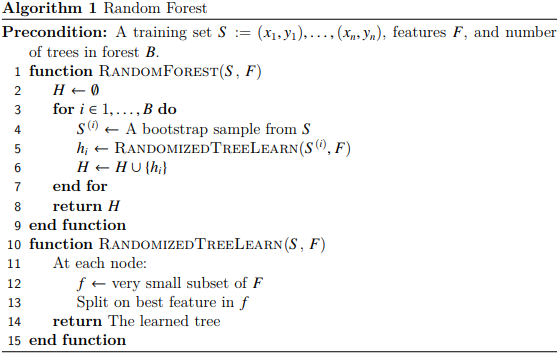
\includegraphics[width=150mm,height=100mm]{figures/pseudocode}
	\caption{Random forest pseudocode}
\end{figure}
\\

As previously mentioned, the algorithm works by creating a forest of decision trees. This means that for B number of trees we take a bootstrap or bagging sample of features from the original data and create these decision trees by splitting the nodes on the best features. Once this has been complete all the way down the trees recursively, we return the finished trees and decide based on majority vote which outcome is the most likely. 
\\
\\
\clearpage
To give a visual representation of a decision tree it would look something like the following:
\begin{figure}[h]
	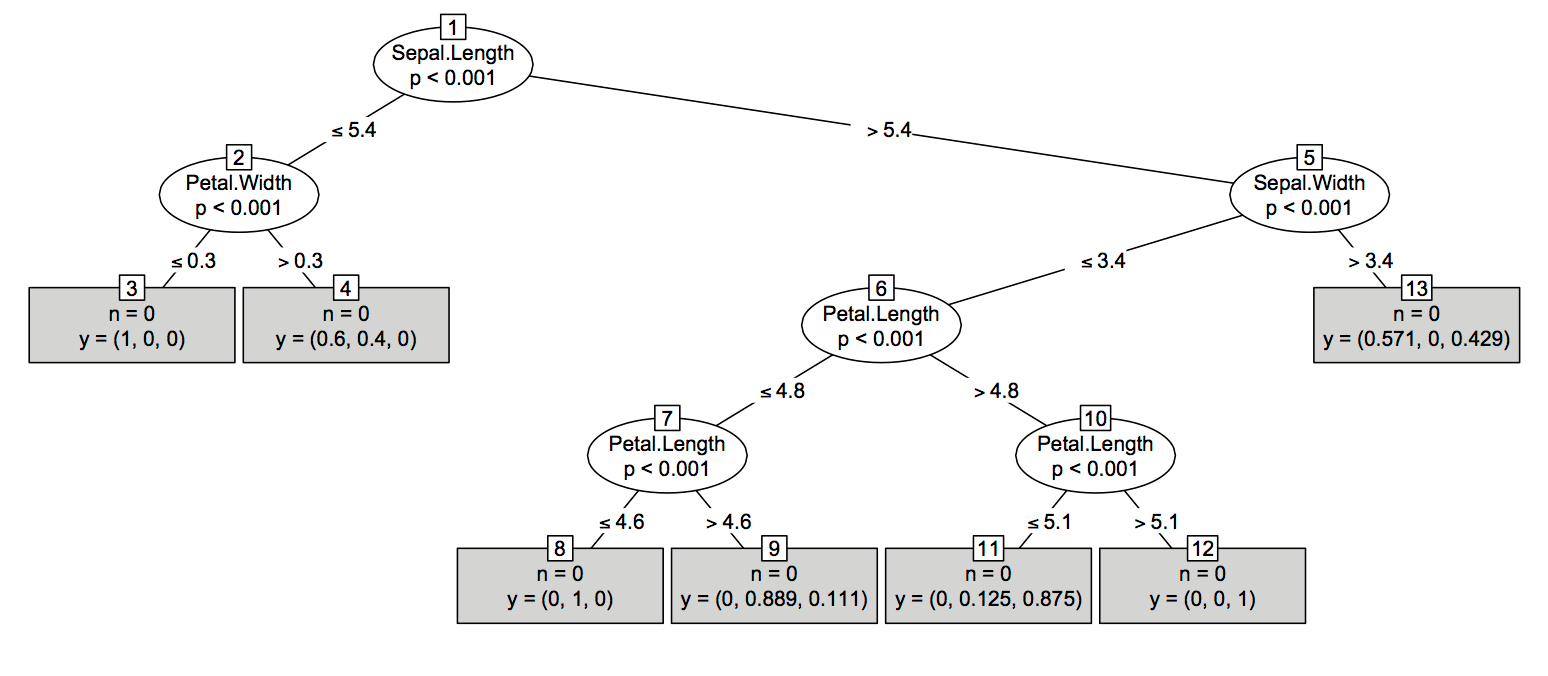
\includegraphics[width=150mm]{figures/tree}
	\caption{An example decision tree using the iris dataset}
\end{figure}
\\
Here you can see that at each node there is a condition being made. This is the 'best' feature that is decided based on the earlier mentioned gini impurity being minimised. Then based on the value of these features for a given datapoint, the algorithm will traverse down a branch of the tree all the way to a root node. This then gives us our prediction for that one decision tree within the forest. 

\section{Deep Learning(Neural Networks)}
Deep learning or more specifically artificial neural networks are a relatively new form of machine learning that is more of a framework than an actual algorithm. ANN's aren't really a specific algorithm, more of a general decision making model. They do not need any sort of rules fed into them or being told what to do. Just some data and it begins training immediately. To understand the basics of ANN's we have to look at what they are made of. An ANN is made up of a multitude of layers. In these layers there are a whole bunch of perceptrons. 
\begin{figure}[!h]
\centering
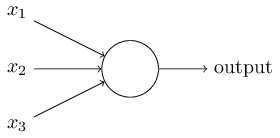
\includegraphics[width=100mm]{figures/perceptron}
\caption{A single perceptron}
\end{figure}

The inputs are summed up with some weights as their coefficients and then compared to a threshold. If greater than said threshold then the output is 1 else it's 0. This rule can be written mathematically such as: 

$$
output = \begin{cases}
0 & \text{ if $\sum_{j}w_{j}x_{j} \leq$ threshold} \\
1 & \text{ if $\sum_{j}w_{j}x_{j}$ > threshold}
\end{cases}
$$

Once you start training your model, the weights $w_{j}$ start to change to match the labels on the training data. As the layers of perceptrons goes on, the more complicated these values are in theory. They aren't just simple decisions any more, but instead represent the decisions made based on all the previous layers too. 



\section{Existing Systems}
There are a handful of algorithms or programs that have been designed to detect these bots. Most of them tend to use a machine learning algorithm as a way to classify accounts and tell them apart from each other, while others have attempted to use deep neural network architectures such as long short-term memory(LSTM).  


\subsection{Tweetbotornot}
\href{https://github.com/mkearney/tweetbotornot}{Tweetbotornot} is a package built in R that uses machine learning to classify Twitter accounts. It has two 'levels'. One for users where it uses information related to an account such as location or number of followers. The other is a tweet-level which checks for details like hashtags, mentions or capital letters out of the user's more recent 100 tweets. 
This could prove useful when testing my program to compare results as the accuracy of this library is 93.8 percent. As this is just a package created, it doesn't have any user-interface program built around it or anything like that, therefore it is unusable by anyone not knowledgable in R. 

\subsection{DeBot}
\href{https://github.com/nchavoshi/debot_api}{DeBot} is a fully functioning python API for bot detection on Twitter. It has the ability to obtain a list of bots already detected by DeBot, or just simply checking individual accounts. You can also get a list of bots which appear in the archives more than a given number of times. They can even be requested based on topics. It does however have a somewhat working built in search mechanism on its \href{https://www.cs.unm.edu/~chavoshi/debot/}{website}.
 
%Chapter 3

\chapter{System Design}

\label{Chapter3}

\section{Method}
The core part of the system will be deciding whether the account it is checking is a bot or not. It will use a form of machine learning to classify the account as either 'bot' or 'not bot'. Initially it would seem as if this was a binary classification issue, however it makes more sense to treat it as a regression problem. This makes it much easier to interpret the results for the user as a probability is easily understood and is a much more honest answer compared to just giving the user a 'yes' or 'no'.


\section{System Requirements}
In order to achieve the aims of the system, there are a few things the program will need to do.
\begin{enumerate}
	\item The system must be able to determine whether an account is a bot or not.
	\item A connection using the Twitter API must be established in order to retrieve users' data.
	\item Allow users to input a Twitter account.
	\item Display the likelihood that an account is a bot or not.
\end{enumerate}




%Chapter 4

\chapter{System Design}

\label{Chapter4}
This chapter is about the methodology behind the program and some of the features and requirements.

\section{Method}
The core functionality of the system is the classification and prediction of said classes. Different machine learning algorithms are used to predict the bots. This task can be treated as either a regression or binary classification problem. In the end the system is a binary predictor therefore the latter makes more sense. 


\section{System Requirements}
In order to achieve the aims of the system, there are a few things the program will need to do.
\begin{enumerate}
	\item The system must be able to determine whether an account is a bot or not.
	\item Display the likelihood that an account is a bot or not.
    \item The system should evaluate the results.
    \item The system should compare results with the other classifiers.
\end{enumerate}

\section{Algorithm}
There are several algorithms in the system running together. These classifiers can be used to compare results with each other to better evaluate them. The different algorithms are; random forest implemented from the ground up and using the sklearn library, as well as an artificial neural network. It's important to keep in mind the accuracy versus the performance of the system. Achieving good results will come due to finding a balance between the two. 


\section{Data}
The data will have to be kept the same throughout for a fair comparison. As it would take an extended period of time to obtain all this data using the system, it's much easier if it uses data already gathered from the internet. 

To start off with, the system will use only numerical data from Twitter accounts, such as number of followers and number of tweets. Using text like the actual content of tweets would be very complicated and most likely require a more complex system then the one designed. If the predictions aren't great then using more or different features can be considered. 

\section{Language}
The language being used to implement the system in it's entirety will be Python. The main reason for selecting this as the language is because of the libraries that can be utilised by it.

\subsection{Sklearn}
Sklearn is a python library designed specifically for machine learning. It has a huge range of supervised and unsupervised learning algorithms. 

\subsection{Keras}
Keras is a high-level neural networks API. It runs on top of tensorflow. It is the basis of the neural network designed for this system. It provides easy to create models that also perform very well and fast.

\subsection{Numpy}
Numpy is a multi-dimensional array package. It's what the system uses for most of its arrays and data manipulation. It allows the system to combine and split multi-dimensional arrays with ease. 

\subsection{Matplotlib}
Matplotlib is only used within the neural network for evaluation of the system. It makes it very simple by drawing plotted graphs of validation accuracy and loss values.















 
%

\chapter{Progress to date}

\label{Chapter5}


%

\chapter{Results}

\label{Chapter6}
This chapter contains the results from all the implementations provided with some assessment of them along with any interesting findings in the process. There will also be comparisons where appropriate as well as trying to figure out why exactly the results are the way they are. 


It's important that before looking at the results there is an acknowledged method of deciding how \textit{good} the results are. 
The first obvious unit of measurement would be accuracy. To see how accurately the designed model predicts the classes of the data. This is the primary value needed to be as high as possible to avoid mistakes. The secondary feature would be time taken to run. This isn't as much of an issue in this experimental setting, however if this sort of system were to be attempted to integrate into other live systems, it is definitely a variable to keep in mind. 
\\
\\
There are a handful of tunable parameters for all the systems designed. To illustrate exactly which systems contain which parameters refer to the following table:


\begin{center}
\begin{tabular}{|c | m{7cm} | c |}
\hline
Parameter & Description & Used in \\
\hline
Number of features & The maximum number of features to be considered when building a tree  & Random forest \& Sklearn \\
\hline
Maximum depth & The maximum depth a tree can have along any path & forest \& Sklearn \\
\hline
Minimum size & The minimum number of nodes required to be present on both sides after a split for it to occur & Random forest \\
\hline
Sample size & The ratio of the subsample that we pick for the bagging process of building a tree & Random forest \\
\hline
Number of trees & The number of trees built in the forest & forest \& Sklearn \\
\hline
Number of folds & The number of folds used in cross validation & Random forest \\
\hline
Epochs & The number of learning cycles done for training & Neural network \\
\hline
Batch size & The number of training examples used in one iteration & Neural network \\
\hline

\end{tabular}
\textit{Table 6.1: Table of tunable parameters}
\end{center}

\section{Random Forest without Sklearn}
The following results are a varying range of accuracies based on some of the parameters being changed around. Most of the parameters have been altered at times to see what difference they make and seeing what combination of parameters give the best results.

Results for random forest implementation without sklearn:
\begin{center}
\begin{tabular}{|c | c | c | c | c | c | c |}
\hline
Trees & Maximum depth & Minimum size & Features & Folds & Sample size & Accuracy \\
\hline
2 & 5 & 1 & $\sqrt{features}$ & 2 & 1.0 & 90.7\% \\
\hline
5 & 5 & 1 & $\sqrt{features}$ & 2 & 1.0 & 92.0\% \\
\hline
10 & 5 & 1 & $\sqrt{features}$ & 2 & 1.0 & 92.4\% \\
\hline
2 & 10 & 5 & $\sqrt{features}$ & 2 & 1.0 & 92.8\% \\
\hline
5 & 10 & 5 & $\sqrt{features}$ & 2 & 1.0 & 96.0\% \\
\hline
10 & 10 & 5 & $\sqrt{features}$ & 2 & 1.0 & 96.1\% \\
\hline
2 & 10 & 1 & $\sqrt{features}$ & 2 & 1.0 & 93.7\% \\
\hline
5 & 10 & 1 & $\sqrt{features}$ & 2 & 1.0 & 96.0\% \\
\hline
10 & 10 & 1 & $\sqrt{features}$ & 2 & 1.0 & 97.3\% \\
\hline
2 & 10 & 1 & $\sqrt{features}$ & 2 & 0.5 & 91.5\% \\
\hline
5 & 10 & 1 & $\sqrt{features}$ & 2 & 0.5 & 95.2\% \\
\hline
10 & 10 & 1 & $\sqrt{features}$ & 2 & 0.5 & 95.4\% \\
\hline
2 & 5 & 1 & $\sqrt{features}$ & 5 & 1.0 & 90.5\% \\
\hline
5 & 5 & 1 & $\sqrt{features}$ & 5 & 1.0 & 92.5\% \\
\hline
10 & 5 & 1 & $\sqrt{features}$ & 5 & 1.0 & 92.3\% \\
\hline

\end{tabular}
\textit{Table 6.2: Table of random forest implementation results}
\end{center}

\subsection{Interpretation of results}
Overall, the results have a good, somewhat expected range based on the other systems researched on the internet. Due to the heavy performance of the system, it was only possible to test the number of trees up to 10. It was clear out of the results that the more trees the better, however this is most likely only the case early on. At some point adding more trees won't really change the overall predictive power of the forest. The tree parameter was one of the two values that had the largest effect on the speed and runtime of the algorithm, with the other being number of folds.

For the maximum depth parameter, out of the two options, the larger one seemed to do a much better job. It's important to keep in mind that adding too much depth to the trees would cause overfitting due to the tree splitting into many paths with very little objects per node. 

When it came to minimum size, changing it from 1 to 5 showed a slight drop in performance. The only beneficial part of increasing this parameter would be in combination with maximum depth. This is due to the minimum size limiting the thin spread out trees from having too many branches with just a few objects going through them. 

The number of features to be considered by the trees was left unchanged because of how small it already was, it would only make the predictions worse. 

The folds' results were quite surprising as increasing the folds actually made the accuracy worse. It's the second parameter that had a huge effect on the speed, due to more folds causing the algorithm to loop that many more times. 

The sample size caused the accuracy to decrease when lowered closer to 0, which is expected as all it does is essentially reduce the number of training data used when building the decision trees.

Overall with all of the results giving at least 90\% accuracy was quite impressive. 




\section{Random Forest with Sklearn}

The following section displays the results from the system built using the sklearn library.
The tests were concluded in similar ways to the other implementation.
The results are as follows:

\begin{center}
\begin{tabular}{| c | c | c | c |}
\hline
Trees & Maximum depth & Features & Accuracy \\
\hline
2 & 10 & $\sqrt{features}$ & 87.3\% \\
\hline
5 & 10 & $\sqrt{features}$ & 88.3\% \\
\hline
10 & 10 & $\sqrt{features}$ & 88.9\% \\
\hline
50 & 10 & $\sqrt{features}$ & 88.8\% \\
\hline
100 & 10 & $\sqrt{features}$ & 89.0\% \\
\hline
500 & 10 & $\sqrt{features}$ & 89.1\% \\
\hline
1000 & 10 & $\sqrt{features}$ & 89.2\% \\

\hline
2 & 20 & $\sqrt{features}$ & 84.9\% \\
\hline
5 & 20 & $\sqrt{features}$ & 87.4\% \\
\hline
10 & 20 & $\sqrt{features}$ & 88.3\% \\
\hline
50 & 20 & $\sqrt{features}$ & 88.4\% \\
\hline
100 & 20 & $\sqrt{features}$ & 88.6\% \\
\hline
500 & 20 & $\sqrt{features}$ & 89.0\% \\
\hline
1000 & 20 & $\sqrt{features}$ & 88.7\% \\
\hline
\end{tabular}

\textit{Table 6.3: Table of sklearn implementation results}
\end{center}


\subsection{Interpretation of results}
The first thing to note about this table is that the range of trees are much higher compared to the previous. This is due to the library running much more efficiently, allowing to create more dense forests with a relatively small amount of time required. There are less tunable parameters here compared to the implementation without sklearn. The accuracies are much closer and there is a slower increase. The overall range is somewhat lower, which is surprising. 

The number of trees has a clear effect on the accuracy just not that much in the later amounts. This is probably due to the fact that there aren't that many features to select from, so most of the later trees end up being duplicates and are predicting the same thing as the other ones. It seems that both systems support the idea that the number of trees make a difference when the overall tree count is quite low. 

Once the system is done training and predicting, it then saves one of the decision trees from the forest as an image so we can see what's happening exactly. An example of that can be seen below:
\begin{figure}[!h]
\centering
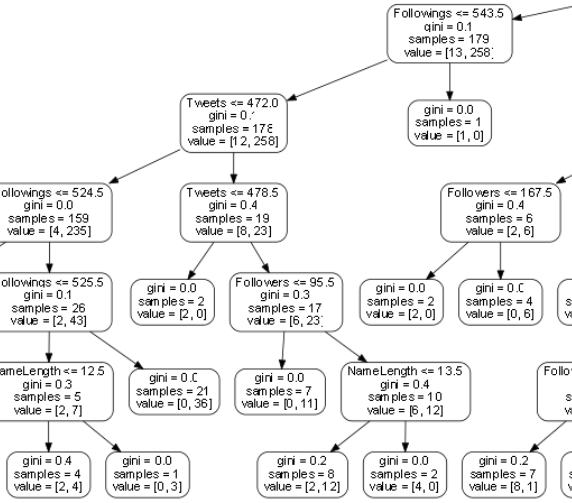
\includegraphics[width=100mm]{figures/decisiontree}
\caption{A section of a decision tree}
\end{figure}

\newpage
\section{Neural Network(NN) model}
The NN model works completely different compared to the random forest algorithms looked at until now. There are only two hyper-parameters, epochs and batch size. NN's tend to overfit after many epochs so it was important to find this point. The strategy was to first run the model for a large amount of epochs and see where the overfitting begins to happen, then only train the model for that specific length to get the best possible prediction.

\newpage

Here are the results of the accuracy and loss for both training and validation sets over 1000 epochs:
\begin{figure}[!h]
    \centering
	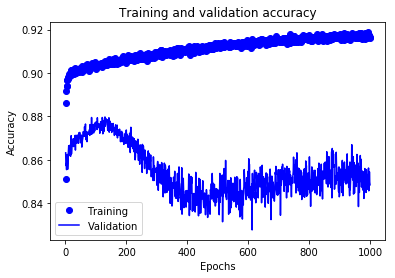
\includegraphics[width=100mm]{figures/accgraph}
	\caption{Accuracy over 1000 epochs}
\end{figure}
\begin{figure}[!h]
    \centering
	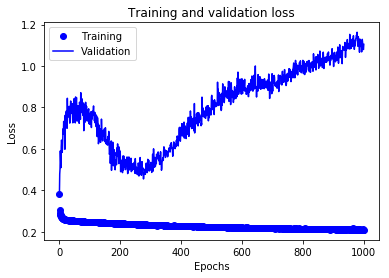
\includegraphics[width=100mm]{figures/lossgraph}
	\caption{Loss over 1000 epochs}
\end{figure}

In \textit{figure 6.1} the accuracy can be seen over the many epochs. The main focus is on the validation plots as that's the part that tells us how good the model is doing predicting new data. Initially the accuracy increases and around 150 epochs it cuts off and starts to decrease. That is roughly the point where overfitting starts to occur. We can confirm this by looking at the loss graph.

When it comes to the other graph, \textit{figure 6.2} we see the loss function, which we are trying to minimise to get rid of the errors. This figure is almost an inverted version of the accuracy one. The validation loss initially shoots up and then begins to decrease as the model is improving itself and adjusting to the data. At around 250 epochs in the validation loss begins to increase indefinitely. This is another major sign of overfitting and is telling us to stop. 

Using these two graphs we need to find a decent stopping point for when we retrain the model with a limited number of epochs then predict the labels of the test data that we put aside from the beginning. 

\begin{figure}[!h]
\centering
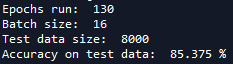
\includegraphics[width=100mm]{figures/nntestpredict}
\caption{Accuracy on test data after 130 epochs}
\end{figure}

\textit{Figure 6.3} shows the result of retraining the model for 130 epochs, then predicting the classes for the test data and comparing it to the actual labels given, which gives us 85.4\% accuracy. This is close to sklearn implementation but quite far off the other one, almost 10\% difference. Overall it's not a bad model as it outperforms randomly assigning the data labels which would result in a basic 50\% accuracy. The good thing about NN is it trains relatively fast and with a lot of data. This means potential future updates would be easy to complete compared to the random forest systems which took much longer. 






%----------------------------------------------------------------------------------------
%	THESIS CONTENT - APPENDICES
%----------------------------------------------------------------------------------------

\appendix % Cue to tell LaTeX that the following "chapters" are Appendices

% Include the appendices of the thesis as separate files from the Appendices folder
% Uncomment the lines as you write the Appendices

% Appendix A

\chapter{Code} % Main appendix title

\label{AppendixA} % For referencing this appendix elsewhere, use \ref{AppendixA}

\section{preprocessing.py}
\begin{lstlisting}
# -*- coding: utf-8 -*-

import numpy as np
import pandas as pd

np.set_printoptions(suppress=True)


def import_data():

    varol_users = np.loadtxt("Z:\ioptyu2\Desktop\gitDissertation\local\Data\\varol_2017.dat")


    col_name = ["UserID","CreatedAt","CollectedAt","Followings","Followers","Tweets","NameLength","BioLength"]
    bot_users = pd.read_csv("Z:/ioptyu2/Desktop/gitDissertation/local/Data/social_honeypot_icwsm_2011/content_polluters.txt",
                                     sep="\t",
                                     names = col_name)


    legit_users = pd.read_csv("Z:/ioptyu2/Desktop/gitDissertation/local/Data/social_honeypot_icwsm_2011/legitimate_users.txt",
                                      sep="\t",
                                      names = col_name)
    
    return [varol_users,bot_users,legit_users,col_name]

#col_name = ["UserID","TweetID","Tweet","CreatedAt"]
#bot_tweets = pd.read_csv("Z:/ioptyu2/Desktop/gitDissertation/local/Data/social_honeypot_icwsm_2011/content_polluters_tweets.txt",
#                                  sep="\t",
#                                  names = col_name)

\end{lstlisting}

\section{random\_forest.py}
\begin{lstlisting}
# -*- coding: utf-8 -*-

from sklearn import datasets
from random import seed
from random import randrange
from math import sqrt
import numpy as np
import preprocessing


iris = datasets.load_iris()

X = iris.data
Y = iris.target
dataset = []
#for i in range(len(X)):
#    dataset.append(np.hstack((X[i],Y[i])))

#cleaning up data(picking out useful rows)
df = preprocessing.import_data()
bots = df[1].values[:2000,3:].astype(int)
legit = df[2].values[:2000,3:].astype(int)


#adding label, bots=1 legit=0
bots = np.hstack((bots,np.ones((bots.shape[0],1))))
legit = np.hstack((legit,np.zeros((legit.shape[0],1))))

dataset = np.vstack((bots,legit))

test_bots = df[1].values[2000:3000,3:].astype(int)
test_legit = df[2].values[2000:3000,3:].astype(int)

test_data = np.vstack((test_bots, test_legit))
test_label = np.vstack((np.ones((test_bots.shape[0],1)), np.zeros((test_legit.shape[0],1))))

#References:
#https://www.python-course.eu/Random_Forests.php
#https://machinelearningmastery.com/implement-random-forest-scratch-python/

#split a dataset into k folds
def cv(dataset,folds):
    dataset_split = list()
    dataset_copy = list(dataset)
    fold_size = len(dataset)/folds
    for i in range(folds):
        fold = list()
        while len(fold) < fold_size:
            index = randrange(len(dataset_copy))
            fold.append(dataset_copy.pop(index))
        dataset_split.append(fold)
    return dataset_split

#calculate accuracy
def accuracy_calc(actual, predicted):
    acc = 0.0
    for i in range(len(actual)):
        if actual[i] == predicted[i]:
            acc += 1.0
    return acc / len(actual) * 100.0

#evaluate the algorithm with cv
def evaluate(dataset, algorithm, folds, *args):
    folds = cv(dataset,folds)
    scores = list()
    for fold in folds:
        train_set = list(folds)
        train_set = sum(train_set, [])
        test_set = list()
        for row in fold:
            row_copy = list(row)
            test_set.append(row_copy)
            row_copy[-1] = None
        predicted = algorithm(train_set, test_set, *args)
        actual = [row[-1] for row in fold]
        accuracy = accuracy_calc(actual, predicted)
        scores.append(accuracy)
    return scores


#split the data into two based on a threshold(value)
def test_split(index, value, dataset):
    left, right = list(), list()
    for row in dataset:
        if row[index] < value:
            left.append(row)
        else:
            right.append(row)
    return left,right

#calculate the gini index
def get_gini(groups, classes):
    instances = float(sum([len(group) for group in groups]))
    gini= 0.0
    for group in groups:
        size = float(len(group))
        if size == 0:
            continue
        score = 0.0
        for class_val in classes:
            p = [row[-1] for row in group].count(class_val) / size
            score += p*p
        gini += (1.0 - score) * (size / instances)
    return gini

#pick the best split 
def best_split(dataset, n_features):
    class_values = list(set(row[-1] for row in dataset))
    b_index, b_value, b_score, b_groups = 999,999,999,None
    features = list()
    while len(features) < n_features:
        index = randrange(len(dataset[0])-1)
        if index not in features:
            features.append(index)
    for index in features:
        for row in dataset:
            groups = test_split(index, row[index], dataset)
            gini = get_gini(groups, class_values)
            if gini < b_score:
                b_index, b_value, b_score, b_groups = index, row[index], gini, groups
    return {'index':b_index, 'value':b_value, 'groups':b_groups}

#create a terminal node value
def terminal(group):
    outcomes = [row[-1] for row in group]
    return max(set(outcomes), key=outcomes.count)

#create child splits for a node or make a terminal
def split(node, max_depth, min_size, n_features, depth):
    left, right = node['groups']
    del(node['groups'])
    #check for no splits
    if not left or not right:
        node['left'] = node['right'] = terminal(left + right)
        return
    #check if max depth
    if depth >= max_depth:
        node['left'], node['right'] = terminal(left), terminal(right)
        return
    #go down left child
    if len(left) <= min_size:
        node['left'] = terminal(left)
    else:
        node['left'] = best_split(left, n_features)
        split(node['left'], max_depth, min_size, n_features, depth + 1)
    #go down right child
    if len(right) <= min_size:
        node['right'] = terminal(right)
    else:
        node['right'] = best_split(right, n_features)
        split(node['right'], max_depth, min_size, n_features, depth + 1)
        

#build a tree
def build_tree(train, max_depth, min_size, n_features):
    root = best_split(train, n_features)
    split(root, max_depth, min_size, n_features, 1)
    return root


#make a prediction using the tree and nodes
def predict(node, row):
    if row[node['index']] < node['value']:
        if isinstance(node['left'], dict):
            return predict(node['left'], row)
        else:
            return node['left']
    else:
        if isinstance(node['right'], dict):
            return predict(node['right'], row)
        else:
            return node['right']


#create a subsample for the data (the bagging/bootstrapping process)
def subsample(dataset, ratio):
    sample = list()
    n_sample = round(len(dataset) * ratio)
    while len(sample) < n_sample:
        index = randrange(len(dataset))
        sample.append(dataset[index])
    return sample

#make a prediction with a list of bagged trees
def bagging_predict(trees, row):
    predictions = [predict(tree, row) for tree in trees]
    return max(set(predictions), key=predictions.count)

#random forest algorithm
def random_forest(train, test, max_depth, min_size, sample_size, n_trees, n_features):
    trees = list()
    for i in range(n_trees):
        #print(i)
        sample = subsample(train, sample_size)
        tree = build_tree(sample, max_depth, min_size, n_features)
        trees.append(tree)
    predictions = [bagging_predict(trees, row) for row in test]
    testing_predictions = [bagging_predict(trees,row) for row in test_data]
    print('Backup testing:', accuracy_calc(test_label, testing_predictions))
    return predictions

#seed
seed(1314)

dataset = np.random.permutation(dataset)


#print results and stuff
n_folds = 2
max_depth  = 10
min_size = 1
sample_size = 1
n_features = int(sqrt(len(dataset[0])-1))
for n_trees in [2,5,10]:
    scores = evaluate(dataset, random_forest, n_folds, max_depth, min_size, sample_size, n_trees, n_features)
    print('Trees: %d' % n_trees)
    print('Scores: %s' % scores)
    print('Mean accuracy: %.3f%%' %(sum(scores)/float(len(scores))))



\end{lstlisting}

\section{sklearnRF.py}
\begin{lstlisting}
# -*- coding: utf-8 -*-
from sklearn.ensemble import RandomForestClassifier
from sklearn.tree import export_graphviz
import pydot
import numpy as np
import preprocessing
from math import sqrt


#1 = bots, 0 = legit
#training data
df = preprocessing.import_data()
train_bots = df[1].values[:12000,3:].astype(int)
train_legit = df[2].values[:12000,3:].astype(int)

feature_list = df[3][3:]

X_train = np.vstack((train_bots,train_legit))

#testing data
test_bots = df[1].values[15000:16000,3:].astype(int)
test_legit = df[2].values[15000:16000,3:].astype(int)

X_test = np.vstack((test_bots,test_legit))

#training labels
train_bots_label = np.ones((train_bots.shape[0],1))
train_legit_label = np.zeros((train_legit.shape[0],1))

Y_train = np.vstack((train_bots_label,train_legit_label))
Y_train = Y_train.ravel(order='C')

#testing labels
test_bots_label = np.ones((test_bots.shape[0],1))
test_legit_label = np.zeros((test_legit.shape[0],1))

Y_test = np.vstack((test_bots_label,test_legit_label))
Y_test = Y_test.ravel(order='C')
a = list()
#random forest algorithm using sklearn
def random_forest(n_trees, max_depth, n_features):
    rf = RandomForestClassifier(n_estimators = n_trees, max_depth = max_depth, max_features = n_features, bootstrap = True)
    rf.fit(X_train, Y_train)
    predictions = rf.predict(X_test)
    save_tree(rf)
    return predictions

#calculate accuracy for predictions
def accuracy(predictions):
#    for i in range(len(predictions)):
#        if predictions[i] < 0.5:
#            predictions[i] = 0.0
#        else:
#            predictions[i] = 1.0
    accuracy = 0.0
    for i in range(len(predictions)):
        if predictions[i] == Y_test[i]:
            accuracy += 1.0
    accuracy = accuracy / len(predictions) * 100
    print("Accuracy: ",accuracy, "%")
    return
#reference for visualisation
#https://towardsdatascience.com/random-forest-in-python-24d0893d51c0

#Visualise a tree
def save_tree(rf):
    tree = rf.estimators_[1]
    export_graphviz(tree, out_file = 'tree.dot', feature_names = feature_list, rounded = True, precision = 1)
    (graph, ) = pydot.graph_from_dot_file('tree.dot')
    graph.write_png('tree.png')
    return


max_depth = 10
n_features = int(sqrt(len(X_test[0])))

for n_trees in [2,5,10,50,100,500,1000]:
    print("Trees: ",n_trees)
    predictions = random_forest(n_trees, max_depth, n_features)
    accuracy(predictions)

\end{lstlisting}

\section{ANN.py}
\begin{lstlisting}
# -*- coding: utf-8 -*-

import numpy as np
import preprocessing
from sklearn.preprocessing import StandardScaler
from keras import layers, models
from keras.utils import to_categorical
import matplotlib.pyplot as plt
from sklearn import datasets



#iris = datasets.load_iris()
#
#X = iris.data
#Y = iris.target
#dataset = []
#for i in range(len(X)):
#    dataset.append(np.hstack((X[i],Y[i])))
#dataset = np.random.permutation(dataset)
#x_train = dataset[:100,:4]
#y_train = dataset[:100,-1]
#
#x_test = dataset[100:120,:4]
#y_test = dataset[100:120,:4]
#
#x_val = dataset[120:,:4]
#y_val = dataset[120:,-1]
#
#y_true = dataset[:,-1]


#############PREPROCESSING##############
df = preprocessing.import_data()
train_bots = df[1].values[:10000,3:].astype(int)
train_legit = df[2].values[:10000,3:].astype(int)

x_train = np.vstack((train_bots,train_legit))


test_bots = df[1].values[12000:16000,3:].astype(int)
test_legit = df[2].values[12000:16000,3:].astype(int)

x_test = np.vstack((test_bots,test_legit))


train_bots_label = np.ones((train_bots.shape[0],1))
train_legit_label = np.zeros((train_legit.shape[0],1))

y_train = np.vstack((train_bots_label,train_legit_label))


test_bots_label = np.ones((test_bots.shape[0],1))
test_legit_label = np.zeros((test_legit.shape[0],1))

y_test = np.vstack((test_bots_label,test_legit_label))
y_true = y_test

val_bots = df[1].values[10000:12000,3:].astype(int)
val_legit = df[2].values[10000:12000,3:].astype(int)

x_val = np.vstack((val_bots, val_legit))

val_bots_label = np.ones((val_bots.shape[0],1))
val_legit_label = np.zeros((val_legit.shape[0],1))

y_val = np.vstack((val_bots_label,val_legit_label))



y_train = to_categorical(y_train)
y_test = to_categorical(y_test)
y_val = to_categorical(y_val)

sc = StandardScaler()
x_train = sc.fit_transform(x_train)
x_test = sc.fit_transform(x_test)
x_val = sc.fit_transform(x_val)

######create model######
model = models.Sequential()
model.add(layers.Dense(64, activation = "relu"))
model.add(layers.Dense(32, activation = 'relu'))
model.add(layers.Dense(2, activation = 'sigmoid'))


model.compile(optimizer = 'adam',
              loss = 'binary_crossentropy',
              metrics = ['accuracy'])

epochs = 100
batch_size = 16

history = model.fit(x_train,
                    y_train,
                    epochs = epochs,
                    batch_size = batch_size,
                    validation_data = (x_val, y_val))


###predictions###
y_pred = model.predict(x_test)

for i in range(len(y_pred)):
    if(y_pred[i][0] < y_pred[i][1]):
        y_pred[i] = 1
    else:
        y_pred[i] = 0
y_pred = y_pred[:,0]

acc = 0.0
for i in range(len(y_pred)):
    if y_pred[i] == y_true[i]:
        acc += 1.0
acc = acc / len(y_pred) * 100
print('Epochs run: ', epochs)
print('Batch size: ', batch_size)
print('Test data size: ', len(y_pred))
print('Accuracy on test data: ', acc, '%')

def comparison_plot(x, 
                    y_A, style_A, label_A, 
                    y_B, style_B, label_B, 
                    title, x_label, y_label):
    
    plt.clf()
    plt.plot(x, y_A, style_A, label = label_A)
    plt.plot(x, y_B, style_B, label = label_B)
    plt.title(title)
    plt.xlabel(x_label)
    plt.ylabel(y_label)
    plt.legend()
    plt.show()

loss = history.history['loss']
val_loss = history.history['val_loss']
comparison_plot(range(1, len(loss) + 1),
                loss, 'bo', 'Training',
                val_loss, 'b', 'Validation',
                'Training and validation loss',
                'Epochs',
                'Loss')

acc = history.history['acc']
val_acc = history.history['val_acc']
comparison_plot(range(1, len(loss) + 1),
                acc, 'bo', 'Training',
                val_acc, 'b', 'Validation',
                'Training and validation accuracy',
                'Epochs',
                'Accuracy')

print("Highest validation accuracy:", val_acc[np.argmax(val_acc)], "Epochs:", np.argmax(val_acc))
print("Lowest validation loss:", val_loss[np.argmin(val_loss)], "Epochs:", np.argmin(val_loss))


\end{lstlisting}


%----------------------------------------------------------------------------------------
%	BIBLIOGRAPHY
%----------------------------------------------------------------------------------------
\printbibliography[heading=bibintoc]




%----------------------------------------------------------------------------------------

\end{document}  
